\subsection{Monotonicity and boundedness}

Before asking whether a sequence has a limit, we can ask how its terms are ordered and whether they remain inside a fixed range.

\begin{definitionbox}[Monotone sequence]
A sequence is increasing if \(a_{n+1}\ge a_n\) for every relevant \(n\), and decreasing if \(a_{n+1}\le a_n\). It is monotone if it is increasing or decreasing.
\end{definitionbox}

\begin{definitionbox}[Bounded sequence]
A sequence is bounded above if there is a number \(M\) such that \(a_n\le M\) for all \(n\). It is bounded below if there is a number \(m\) such that \(m\le a_n\) for all \(n\).
\end{definitionbox}

\begin{examplebox}[A decreasing bounded sequence]
For
\[
a_n=\frac1n,
\]
we have \(a_{n+1}<a_n\), so the sequence is decreasing. Also \(0<a_n\le1\), so it is bounded below by \(0\) and above by \(1\).
\end{examplebox}

\begin{examplebox}[An increasing unbounded sequence]
For
\[
b_n=n,
\]
we have \(b_{n+1}>b_n\), so the sequence is increasing. It is bounded below, but it is not bounded above.
\end{examplebox}

\begin{examplebox}[Bounded but not monotone]
The sequence
\[
c_n=(-1)^n
\]
alternates between \(-1\) and \(1\). It is bounded, but it is neither increasing nor decreasing.
\end{examplebox}

\begin{center}
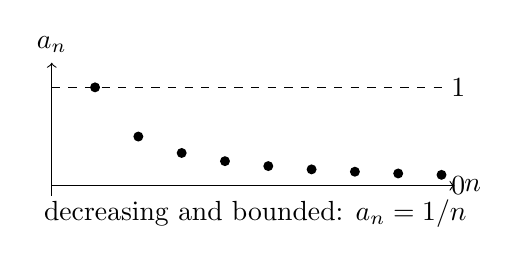
\begin{tikzpicture}[x=0.55cm,y=1.25cm]
  \draw[->] (0,0) -- (9.3,0) node[right] {$n$};
  \draw[->] (0,-0.1) -- (0,1.25) node[above] {$a_n$};
  \draw[dashed] (0,1) -- (9,1) node[right] {$1$};
  \draw[dashed] (0,0) -- (9,0) node[right] {$0$};
  \foreach \n in {1,...,9} {
    \fill (\n,{1/\n}) circle (1.8pt);
  }
  \node at (4.7,-0.28) {decreasing and bounded: $a_n=1/n$};
\end{tikzpicture}

\vspace{0.8em}

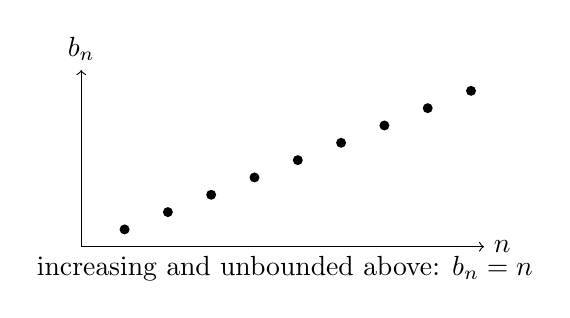
\begin{tikzpicture}[x=0.55cm,y=0.22cm]
  \draw[->] (0,0) -- (9.3,0) node[right] {$n$};
  \draw[->] (0,0) -- (0,10.2) node[above] {$b_n$};
  \foreach \n in {1,...,9} {
    \fill (\n,\n) circle (1.8pt);
  }
  \node at (4.7,-1.25) {increasing and unbounded above: $b_n=n$};
\end{tikzpicture}

\vspace{0.8em}

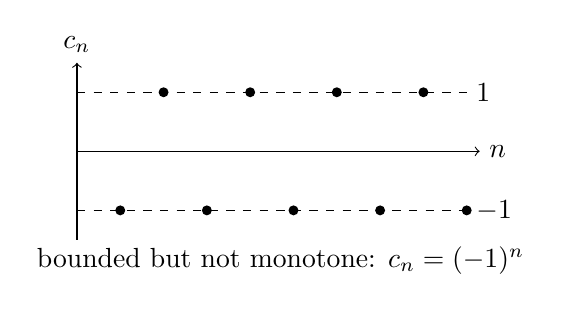
\begin{tikzpicture}[x=0.55cm,y=0.75cm]
  \draw[->] (0,0) -- (9.3,0) node[right] {$n$};
  \draw[->] (0,-1.5) -- (0,1.5) node[above] {$c_n$};
  \draw[dashed] (0,1) -- (9,1) node[right] {$1$};
  \draw[dashed] (0,-1) -- (9,-1) node[right] {$-1$};
  \foreach \n in {1,...,9} {
    \pgfmathsetmacro{\y}{(-1)^\n}
    \fill (\n,\y) circle (1.8pt);
  }
  \node at (4.7,-1.85) {bounded but not monotone: $c_n=(-1)^n$};
\end{tikzpicture}
\end{center}

\begin{interpretationbox}[Reading the three pictures]
The first sequence moves in one direction and remains trapped between two horizontal levels. The second also moves in one direction, but it escapes every proposed upper bound. The third remains trapped, yet repeatedly changes direction. The pictures show that monotonicity and boundedness answer different questions.
\end{interpretationbox}

\begin{interpretationbox}[Preparing the limit question]
Monotonicity describes direction; boundedness describes confinement. Together they give strong information about long-term behavior, but neither property alone is the same as convergence.
\end{interpretationbox}
